\section{Prologue}
This course was originally developed by Dr Wayne Stewart (formerly of The
University of
Auckland) and was first offered in 2009 (Figure~\ref{fig:wayne}).
I joined the faculty in July 2012
and took over the course from him. Wayne is a passionate Bayesian and advocate
for the inclusion of Bayesian statistics in the undergraduate curriculum.
While this edition of the course differs from Wayne's in some ways
\footnote{The differences are mostly cosmetic. 90\% of the content is the same.}
, I hope I am able to do the topic justice in an accessible way.

In this course we will use the following software:
\begin{itemize}
\item R ({\tt http://www.r-project.org/}) \\
\item JAGS ({\tt http://mcmc-jags.sourceforge.net/}) \\
\item R-Studio ({\tt http://www.rstudio.org/})
\end{itemize}
In the labs, our preferred editor will be R-Studio, although any text editor
can be used in principle. These programs are all free and open source software.
That is, they are free to use, share and modify. They should work on
virtually any operating system including the three most popular:
Microsoft Windows, Mac OS X and GNU/Linux. In previous editions of the course,
WinBUGS was used instead of JAGS. However, WinBUGS has not been updated for
several years, and only works on Microsoft Windows. The differences between
the two are fairly minor.

\subsection{Bayesian and Classical Statistics}
Throughout this course we will see many examples of Bayesian analysis, and we
will sometimes mention or allude to the result from {\it classical} or
{\it frequentist} statistics, which is the other way of doing things. You will
have seen some classical statistics methods from STATS 10X and 20X, and
possibly other courses as well.

Many
people have differing views on the status of these two ways of doing statistics.
In the past, Bayesian statistics was controversial, and you had to be very
brave to use it! Many people were {\bf anti}-Bayesian. Those people are now
rare: instead of Bayesians and anti-Bayesians, it would be more realistic to
say there are now Bayesians and non-Bayesians, and many of the non-Bayesians
would be happy to use Bayesian statistics in some circumstances.
The non-Bayesians would say that
Bayesian statistics is {\it one way} of doing things, and it is a matter of
choice which ways you prefer to use. In my opinion, Bayesian
statistics is {\it the right way} to do things, and non-Bayesian methods are
always, at least subtly, wrong, even if they perform well in practice (which
they often do). There is one point that you should keep in mind throughout
this course, though, and it is very important:
{\bf You do not have to agree with me in order to do well in this course!}

\begin{figure}
\begin{center}
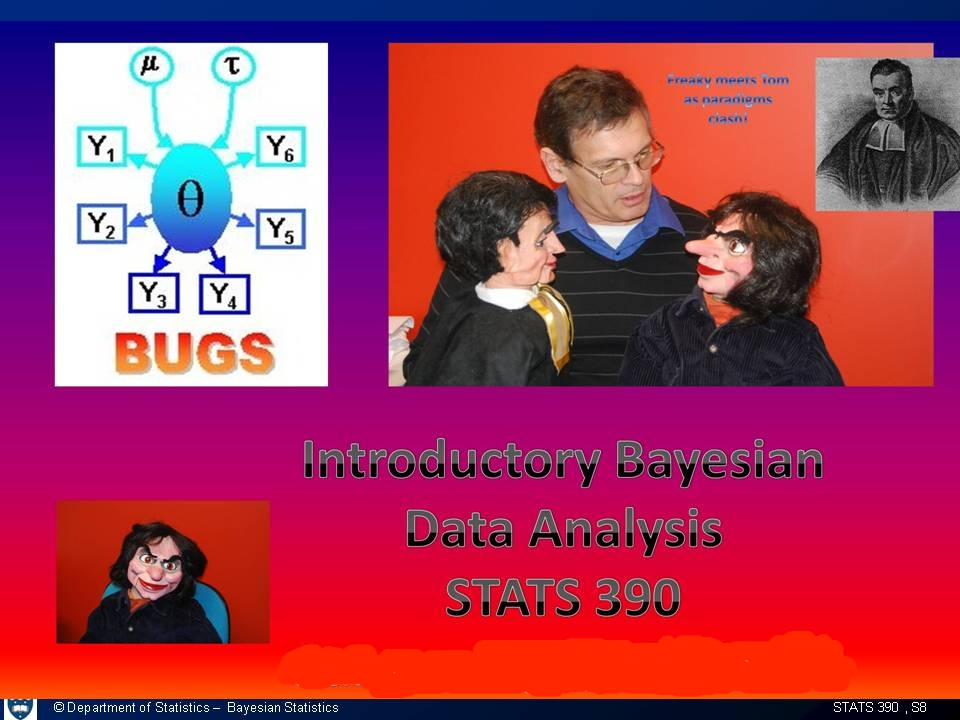
\includegraphics[scale=0.5]{390course.jpg}
\end{center}
\caption{An ad for the original version of this course (then called
STATS390), showing Wayne Stewart with two ventriloquist dolls, who would
have debates about statistics.\label{fig:wayne}}
\end{figure}

\subsection{List of Bayesian Statistics Terminology}
Prior probability, posterior probability, prior distribution, posterior
distribution, markov chain monte carlo (MCMC) methods

\subsection{List of Classical/Frequentist Statistics Terminology}
Estimator, Confidence Interval, p-value, bias, bootstrap.

